\chapter{実験}
\label{chap:experiment}
第4章で述べた提案手法の有効性を検証するために,BAIR Push Datasetという行動条件付き映像予測用のデータセットを用いて評価実験を行った.本章では実験の内容について説明した後に実験結果について述べる.

\section{実験内容}
第4章で述べた提案手法とベースラインの比較を行う.ベースラインは第二章で述べたシンプルなDSSMとし,状態ベクトルの次元を64, 128, 256, 512, 1024の6通りに変えて実験を行う.提案手法は64次元と512次元の二階層の状態ベクトルを持つモデルと,64次元と512次元と4096次元の三階層の状態ベクトルを持つモデルとした.ベースラインと提案手法の実装の差は必要最小限にとどめ,どちらも学習時には10フレーム先までの予測を行った.またパラメータの最適化にはそれぞれ確率的勾配降下法アルゴリズム Adam[引用] を用いた.
評価指標には,定量評価として予測誤差(負の対数尤度)を測り,合わせて定性評価も行う.またこれらの評価時には,DSSMと同じデコーダー・エンコーダーモデルを持つVAEを用意し,時系列方向の遷移を学習する必要がない場合の生成モデルの精度とも比較を行う.(この実験自体TODO.)

\subsection{データセット}
(TODO: データセットを紹介する図を入れる)

今回用いるBAIR Push Datasetは行動条件付き映像予測と行動条件をつけない映像予測のどちらの研究でも用いられるデータセットであり,カリフォルニア大学バークレー校によって制作・公開されている.[引用]
こちらのデータセットは,様々な物体がおかれた机の上をロボットアームがランダムに掻き乱すようにして様々なデータが記録されており,今回はその中から行動系列$\vec{a}$と固定視点から観測された画像系列$\vec{o}$を用いる.今回用いる行動系列$\vec{a}$は,具体的にはロボットのエンドエフェクタの位置姿勢の命令値になっている.観測画像は64x64サイズのRGB画像で,これらのデータは10hzで撮られている.

\subsection{ベースラインの実装}
実装にはFacebook社製の深層学習フレームワークであるPytorch[引用]と,松尾研究室研究員の鈴木さんが中心となって開発されている深層生成モデルライブラリPixyz[引用]を主に用いた.学習用データの読み込みとその最適化にはGoogle社製の深層学習フレームワークであるTensorFlow[引用]を用いた.また実装では,DSSMを用いた強化学習手法であるPlaNetの公開実装[引用]を参考にした.
まずベースラインの実装を説明した後,提案手法の実装について述べる.

\subsubsection{モデルアーキテクチャ}
ベースラインは4つの部分モデルから構成される.
\begin{itemize}
    \item デコーダー $p(s_t|x_t)$
    \item エンコーダー $q(x_t|h_t)$
    \item 遷移モデル(事前分布) $p(s_t|s_t-1, a_t)$
    \item 遷移モデル(事後分布) $q(s_t|s_t-1, a_t, h_t)$
\end{itemize}

遷移モデル(事前分布)とデコーダーが生成モデルに相当し,提案手法のグラフィカルモデルの実践部分を表しす.遷移モデル(事後分布)とエンコーダーが推論モデルに相当し,提案手法のグラフィカルモデルの点線部分を表している.

\begin{description}
    \item[デコーダー・エンコーダー]\mbox{}\\
(図TODO)
PlaNetに倣い,デコーダー/エンコーダーモデルにはWorldModel(Ha 2018)の論文中に記載されているモデルを採用した.デコーダーは各時刻の状態ベクト$s_t$を全結合層で1024次元の隠れ変数に変換したあと,4層の逆畳み込み層で観測画像と同じサイズである64x64サイズのRGB画像に変換する.出力は各ピクセルごとに正規分布をおくが,本研究では簡単のためその分散はそれぞれ1に固定している.
エンコーダーは各時刻の観測を4層の畳み込み層と1層の全結合層で1024次元の隠れ変数$h_t$に変換する.

本研究では,状態変数の次元を変えた際にも隠れ層のパラメータ数などは一切変えなかった.

    \item[遷移モデル]\mbox{}\\
(図TODO)
遷移モデルには,ある時刻の状態ベクトル$s_t$を生成過程に従って生成する事前分布モデルと,ある時刻の観測$o_t$も与えられたときに$s_t$を推論する事後分布モデルの2種類を用意する.

この2つのモデルはアーキテクチャはほとんど共通で入力とするデータだけが違い,事前分布モデルでは一つ前の時刻の状態$s_{t-1}$と行動$a_t$を入力とするが事後分布ではそれに加えその時刻の観測$o_t$をエンコードして得たデータ$h_t$を入力とする.出力はどちらのモデルも次の時刻の状態ベクトルの分布の母数(平均と標準偏差)である.
アーキテクチャは,入力情報をすべて連結して一度全結合層で変換したものを平均を求める全結合層と標準偏差を求める全結合層のそれぞれで変換し,求めたい分布の平均と標準偏差を出力する.

\end{description}

\subsubsection{学習の安定化}
潜在変数の次元を大きくした際,学習の初期段階でカルバックライブラー距離の計算値が発散することがよく起こる.これは遷移モデルが次の時刻の状態ベクトルの分布の標準偏差として0に非常に近い値を出力してしまった結果(丸め誤差が発生して)カルバックライブラー距離の計算時にゼロ除算が発生してしまうためである.この問題は遷移モデルが出力する標準偏差に下限を設けることで解決することができる.今回の実験では潜在変数の次元を1024次元にした際にこのカルバックライブラー距離が学習開始後直ちに発散する問題が発生したので,標準偏差の下限値を$10^{-7}$とすることで学習をある程度継続することができた.ただし標準偏差に下限を設けることは経験的に学習を難しくすることがわかっていたので,他の条件での実験の際には適用しなかった.

\subsection{提案手法の実装}
提案手法はベースラインの節で説明した部分モデルをほぼそのまま用いる.二階層目以上の第i層では,各遷移モデルの入力として一時刻前の状態変数$s^i_{t-1}$と行動$a_t$だけでなく,一つ低次元の層の同じ時刻の状態ベクトル$s^{i-1}_t$も入力とする.また,提案手法では,パラメータを固定している層の状態ベクトルのサンプリングには,モデルの評価時の設定に合わせて常に事前分布を用いている.これは,パラメータを固定している層はそれ以上学習されないために,事前分布より良い表現が下の階層に渡されることはなく,むしろ事前分布で足りない表現を積極的に下の階層の学習で獲得できるようにするためである.
その他はベースラインの実装と変えていない.


\section{実験結果}
TODO
\subsection{定量評価(尤度)}

\begin{figure}[tbp]
\begin{center}
    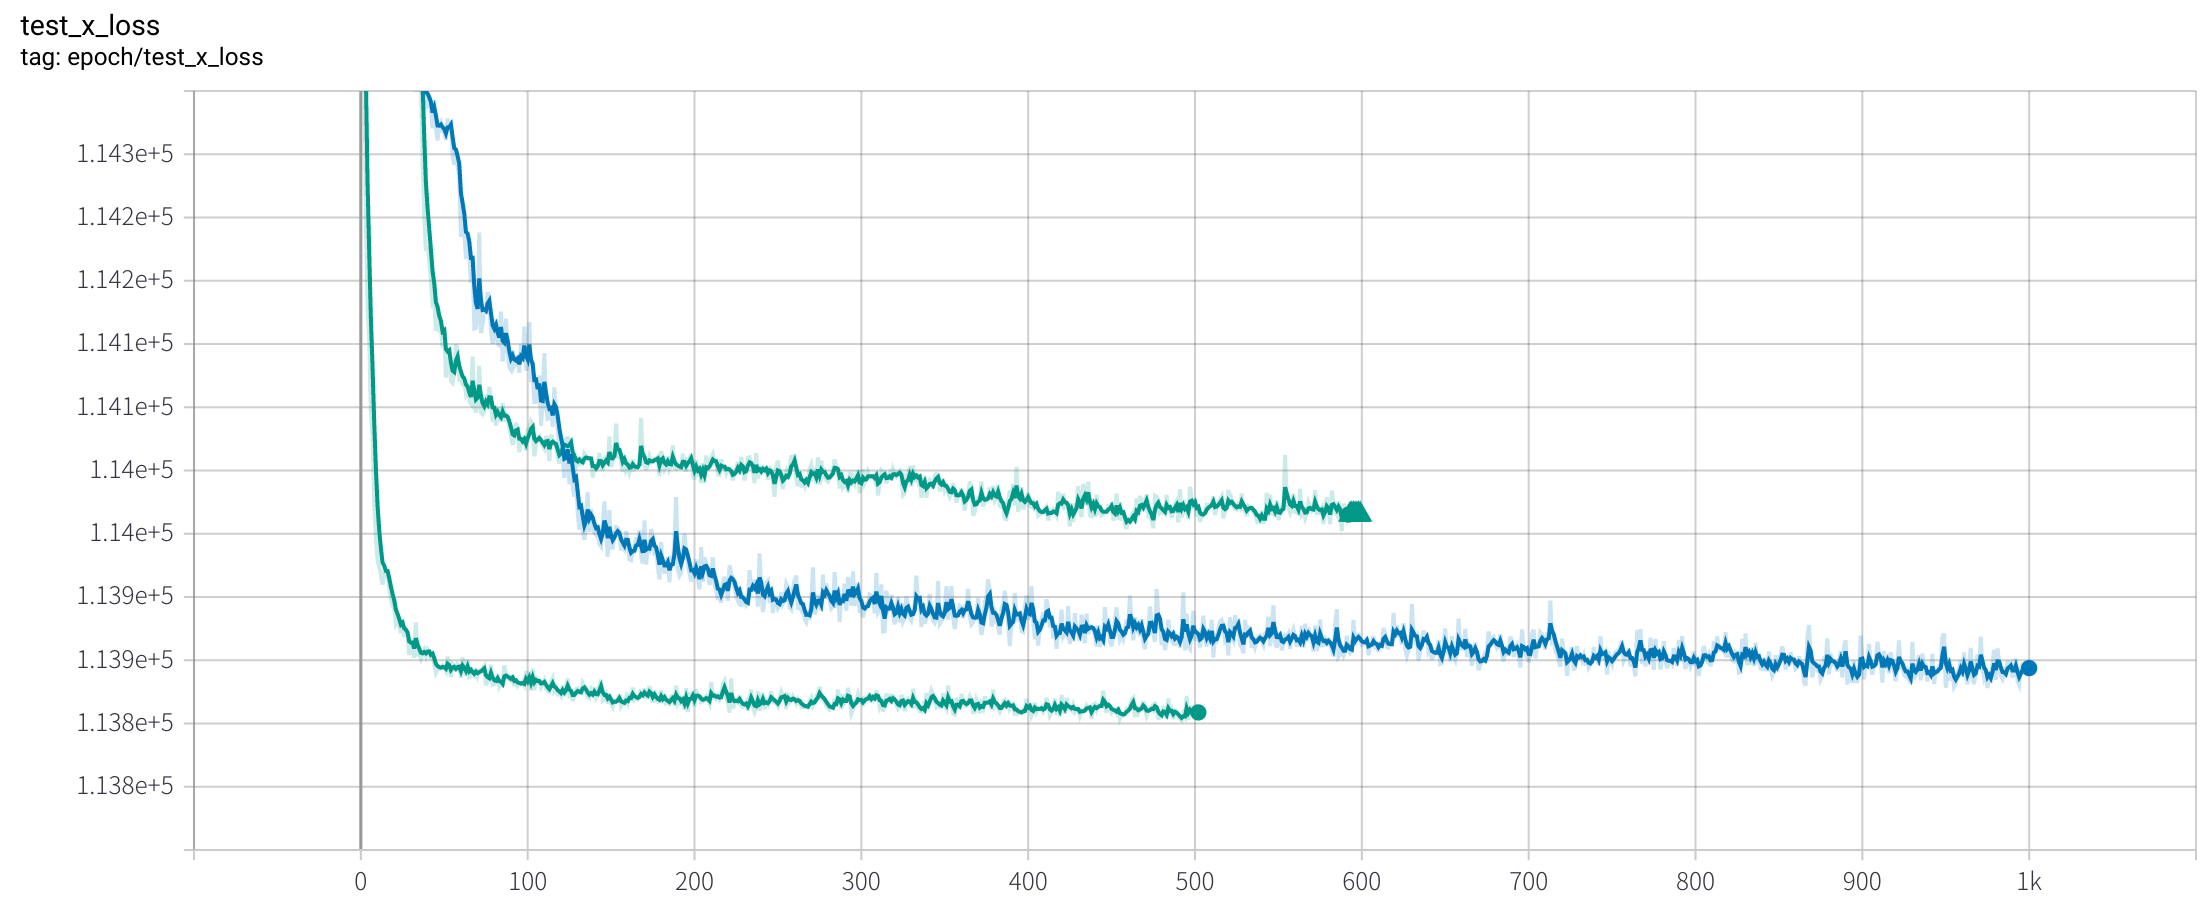
\includegraphics[width=\linewidth]{./figures/proposal_curve}
    \caption[提案手法の学習曲線]{提案手法の学習曲線 一番下が提案手法.TODO: 綺麗にする,凡例入れる}
    \label{fig:vae_example}
\end{center}
\end{figure}

上から
\begin{itemize}
    \item ベースライン(512次元)
    \item ベースライン(64次元)
    \item 提案手法(64 + 512次元)
    \item (提案手法(64 + 512 + 4096次元)(実験待ち))
\end{itemize}

安定した.

尤度上は改善した

定性的に改善したとはいい難い結果になった..

高次元で学習できるようになった.これは深層状態空間モデルの大きな問題点を克服できたと言える.

潜在変数のサンプリングが安定し,学習が簡単になったためだと考える.

\subsection{定性評価}
